\newcommand{\vect}[1]{\mathbf{#1}}
\newcommand{\mat}[1]{\mathbf{#1}}

\newcommand{\pos}{\vect{x}}
\newcommand{\dx}{\vect{\Delta x}}
\newcommand{\xcur}{\vect{x}_{n}}
\newcommand{\xnext}{\vect{x}_{n+1}}
\newcommand{\vel}{\vect{v}}
\newcommand{\dv}{\vect{\Delta v}}
\newcommand{\vcur}{\vect{v}_{n}}
\newcommand{\vnext}{\vect v_{n+1}}
\newcommand{\acc}{\vect{a}}
\newcommand{\force}{\vect{f}}
\newcommand{\forcext}{\vect{f}_{ext}} 
\newcommand{\lam}{\vect{\lambda}}
\newcommand{\lcur}{\lam_{n}}
\newcommand{\lnext}{\lam_{n+1}}
\newcommand{\avlam}{\bar{\lam}}
\newcommand{\fcur}{\vect{f}_{n}}
\newcommand{\fnext}{\vect f_{n+1}}
\newcommand{\M}{\mat M}
\newcommand{\Minv}{\mat M^{-1}}
\newcommand{\Mbinv}{\bar{\mat M}^{-1}}
\renewcommand{\P}{\mat P}
\newcommand{\I}{\mat I}
\newcommand{\J}{\mat J}
\newcommand{\Jt}{\mat J^T}
\newcommand{\C}{\mat C}
\newcommand{\D}{\mat D}
\newcommand{\K}{\mat K}
\newcommand{\violation}{ \phi}
\newcommand{\dviolation}{\dot \violation}
\newcommand{\violcur}{\violation_{n}}
\newcommand{\dviolcur}{\dot \violcur}
\newcommand{\violnext}{\violation_{n+1}}
\newcommand{\dviolnext}{\dot \violation_{n+1}}
\newcommand{\cmp}{c}
\newcommand{\dampingratio}{d}

\section{Introduction}
This plugin serves two purposes:
\begin{itemize}
 \item to provide a new, more complete mechanisme for assembling the dynamical system matrices such as mass $\M$ and stiffness $\K$, as well as constraint Jacobians $\J$,
 \item and experiment a unified approach of soft and hard constraints, inspired from~\cite{servin2006interactive}.
\end{itemize}
Contrary with other implementations of matrix assembly available in SOFA, this one handles mappings, and even multimappings.

Sections \ref{sec constraint forces} and \ref{sec:time integration} explain the unified constraint approach, while Section~\ref{sec matrix assembly} presents the matrix assembly process based on an example. An overview of the corresponding API is given in Section~\ref{sec implementation}. 

\section{Constraint forces} \label{sec constraint forces}
This approach unifies soft and hard constraints, by providing constraints with compliance. 
\subsection{Hard constraints}
For a good introduction on hard constraints, see~\cite{witkinconstraints}.
Hard constraints are usually implemented using Lagrange multipliers $\lambda$ in the following equation:
\begin{equation} \label{eq acc hard}
\left( \begin{array}{cc}
\M & -\Jt \\
 \J &  \end{array}\right)
\left( \begin{array}{c}
\acc \\ \lam
\end{array}\right) = \left( \begin{array}{c}
\forcext  \\
-\ddot \violation
\end{array}\right) 
\end{equation}
where $\M$ is the mass matrix (or, more generally, a dynamics matrix such as $\M-h²\K$ used in implicit time integration), $\J$ is the Jacobian matrix of the constraint(s), $\acc$ is the acceleration, $\forcext$ is the net external force applied to the system, $\lam$ is the constraint force $\violation$ is the constraint violation and $\ddot \violation$ is the second time derivative of the violation (i.e. the error on accelerations).
This form of equation system is typically called \textit{Karush-Kuhn-Tucker (KKT)}.
$\lam$ and $\ddot \violation$ are vectors with as many entries as scalar constraints. The equation system is typically solved using a Schur complement to compute the constraint forces:
\begin{equation}\label{eq schur rigid}
\J \Minv \Jt \lam = -\ddot \violation - \J \Minv \forcext
\end{equation}
and then the acceleration is computed as $\acc = \Minv( \forcext + \Jt \lam)$.

\subsection{Projective constraints}
When the constraints are simple enough, such as keeping points fixed or in some hyperplane, they are more easily handled by straightforwardly projecting forces and displacements.
The previous equation becomes:
\begin{equation} \label{eq acc hard projected}
\left( \begin{array}{cc}
\P\M & -\P\Jt \\
 \J\P &  \end{array}\right)
\left( \begin{array}{c}
\acc \\ \lam
\end{array}\right) = \left( \begin{array}{c}
\P\forcext  \\
-\ddot \violation
\end{array}\right) 
\end{equation}
 where $\P$ is the orthogonal projection matrix corresponding to the constraint.

\subsection{Generalized constraints}
In the generalized approach, the constraint forces are considered directly proportional to the constraint violations $\violation$ and their first time derivative (error on velocity) $\dviolation$:
\begin{equation}\label{eq generalized constraint}
\lam = - \frac{1}{\cmp} \left( \violation + \dampingratio \dviolation \right)
\end{equation}
where the positive real number $\cmp$ is the compliance of the constraint and $\dampingratio$ is its damping ratio.
Combined with a time discretization scheme, this leads to an equation system similar to \eqref{eq schur rigid} as shown in Section~\ref{sec:time integration}.
% This leads to equation system:
% \begin{equation} \label{eq acc compliant}
% \left( \begin{array}{cc}
% \M & -\Jt \\
%  \J &  \C \end{array}\right)
% \left( \begin{array}{c}
% \acc \\ \lam
% \end{array}\right) = \left( \begin{array}{c}
% \forcext  \\
% -\violation - \dampingratio \dviolation
% \end{array}\right) 
% \end{equation}
% where $\C$ is the compliance matrix, typically diagonal, which is null for hard constraints. The corresponding Schur complement is well-conditioned for hard constraints:
% \begin{equation}\label{eq schur compliant}
% \left( \J \Minv \Jt  +   \C \right) \lam = -\violation - \dampingratio\dviolation - \J \Minv \forcext
% \end{equation}
% contrary to the standard implicit integration approach, where the indefinite stiffness matrix grows to infinity for hard constraints.

\subsection{Force or constraint ?} \label{sec force or constraint}
ForceFields usually contribute the the top line of Equation~\ref{eq acc hard}, by accumulating force in the right-hand term. In implicit integration, their stiffness matrix is also accumulated to the left-hand side.
When a ForceField has an invertible stiffness matrix, it can alternatively be handled as a constraint with non-null compliance, rather than a standard force. In this case, it contributes to the bottom of Equation~\ref{eq acc hard} rather than to the top.

Due to matrix conditioning issues, and depending on which linear solver is used, it may be a good idea to process very stiff forces as low compliances rather than large stiffnesses. 
In this case, we call them \textit{compliant} or \textit{compliance forces}. Here the term compliant does not convey information on the magnitude of the stiffness (or compliance) but only on the way it is processed by the solver, namely in the bottom row of the KKT equation system.
Note, however, that each force handled as a constraint increases the size of the equation system, since it adds lines to the bottom (and columns to the right) of the equation system.
Conversely, it may be more efficient to handle soft forces as stiffnesses, since the size of the stiffness matrix depends on the number of independent DOFs, which does not increase along with the number of forces. We call such forces \textit{stiff} or \textit{stiffness forces}, though here again, the term does not convey information on the magnitude of the stiffness but only on the way it is handled by the solver, namely in the first row of the KKT equation system.

Note that geometric stiffness is not (yet) handled in the compliance view, which may result in instabilities in case of large displacements.


\section{Time integration} \label{sec:time integration}
Our integration scheme is:
\begin{eqnarray}
 \vnext &=& \vcur + h \Minv \left(\alpha \fnext + (1-\alpha) \fcur\right) \label{eq ode velocity} \\
  \xnext &=& \xcur + h \left( \beta \vnext + (1-\beta) \vcur \right) \label{eq ode position}
\end{eqnarray}
where index $n$ denotes current values while index $n+1$ denotes next values, $\alpha$ is the implicit velocity factor, and $\beta$ is the implicit position factor. Let
\begin{eqnarray}
 \dv = \vnext -    \vcur  &=& h \Minv \left(\alpha \fnext + (1-\alpha) \fcur\right) \\
\dx = \xnext -  \xcur    &=& h (v + \beta  \dv)
\end{eqnarray}
be the velocity and position changes across the time step.
We have not carefully studied the influence of these parameters, but it seems that $\alpha=0.5$ and $\beta=1$ corresponds to an \textbf{energy-conserving integration scheme}.


The constraint violation $\violation$ and its Jacobian $\J$ are:
\begin{eqnarray}
 \J &=& \frac{\partial \vect \violation}{\partial \pos} \\
 \violnext &\simeq& \violcur + \J \dx = \violcur + h   \dviolation + \J h \beta \Delta \vel  \label{eq violnext}\\
\dviolnext &\simeq& \dviolcur + \J \dv \label{eq dviolnext}
\end{eqnarray}
The corresponding forces are:
\begin{eqnarray}
 \force &=& \forcext + \Jt \lam \\
 \lam_i &=& -\frac{1}{c_i} (  \violation_i + d \dviolation_i ) \label{eq lambda}
\end{eqnarray}
where the subscript $i$ denotes a scalar constraint.

The average constraint forces are computed  using equations \ref{eq lambda}, \ref{eq violnext} and \ref{eq dviolnext}:
\begin{eqnarray*}
 \avlam_i &=& \alpha \lnext + (1-\alpha) \lcur \\
&=& -\frac{1}{c_i} ( \alpha \violation + \alpha h \dviolation  + \alpha h \beta \J \Delta \vel + \alpha d \dviolation + \alpha d \J \dv + (1-\alpha)\violation + (1-\alpha) d \dviolation  ) \\
&=& -\frac{1}{c_i} ( \violation + d\dviolation + \alpha h \dviolation + \alpha(h\beta+d)\J \dv )
\end{eqnarray*}
We can rewrite the previous equation as:
\begin{equation} \label{eq bottom}
 \J \dv + \frac{1}{\alpha(h\beta+d)}\C\avlam = - \frac{1}{\alpha(h\beta+d)} (\violation + (d+\alpha h)\dviolation)
\end{equation}
where values without indices denote current values.
The complete equation system has the following generalized KKT form:
\begin{equation}
 \left( \begin{array}{cc}
\frac{1}{h}\P\M & -\P\Jt \\
\J & \frac{1}{l} \C \end{array}\right)
\left( \begin{array}{c}
\dv \\ \avlam
\end{array}\right) = \left( \begin{array}{c}
\P\forcext  \\
- \frac{1}{l} (\violation +(d+\alpha h) \dviolation)
\end{array}\right) 
\end{equation}
where $ l=\alpha(h \beta + d) $
The system is singular due to matrix $\P $, which removes independent degrees of freedom without reducing the size of the mass matrix accordingly.
To remedy this, we set an option to replace it with 
\begin{equation} \label{eq mbar}
\bar\M = \P \M \P^T + diag(\epsilon),
\end{equation}
 where $\epsilon$ is a very small number. 
This makes the matrix PSD, and does not significantly change the value of the equation solution thanks to the small magnitude of the perturbation.

% \[ \begin{array}{ccc}
% \left( h\J\P\Minv\P\Jt + \frac{1}{l}\C \right) \avlam &=& -\frac{1}{l} \left(\violation + (\dampingratio+h\alpha)\dviolation \right) - h\J \Minv \forcext \\
% \dv &=& h\P\Minv(\forcext +\Jt \avlam ) \\
% \dx &=& h( \vel + \beta \dv )
% \end{array} \]

By inverting $\bar\M$, we can insert the first line of the equation system and get:
\begin{equation} \label{eq schur complement}
 \left( h\J\Mbinv\Jt + \frac{1}{l}\C \right) \avlam = -\frac{1}{l} \left(\violation + (\dampingratio+h\alpha)\dviolation \right) - h\J \P^T \Mbinv \forcext
\end{equation}
where matrix $ h\J\Mbinv\Jt + \frac{1}{l}\C $ is called the Schur complement of the KKT equation system.
Solving for $\avlam$ allows us to update the velocities and the positions:
\begin{eqnarray}
 \dv &=& h\P\Mbinv(\forcext +\Jt \avlam ) \label{eq update velocities}\\
\dx &=& h( \vel + \beta \dv ) \label{eq update positions}
\end{eqnarray}



\section{Matrix assembly} \label{sec matrix assembly}
The equation system, in its most general form, can be written as:
\begin{equation}
 \label{eq abstract system}
 \left( \begin{array}{cc}
\M & -\Jt \\
\J &  \C \end{array}\right)
\left( \begin{array}{c}
\pos \\ \lam
\end{array}\right) = \left( \begin{array}{c}
\force  \\
\violation
\end{array}\right) 
\end{equation}
We assemble the $7$ terms of equation~\ref{eq abstract system} separately. 

Figure~\ref{fig system graph} shows an example of mechanical system.
The independent DOFs are $X_{a}$ and $X_d$.
State $X_b$ is attached to $X_a$ using a simple mapping, and a mass matrix $M_{bb}$ is defined at this level.
State $X_c$ is attached to $X_b$ using a simple mapping, and a compliance matrix $C_{\alpha \alpha}$ (possibly a deformation force) is applied to these DOFs.
State $X_e$ is attached to $X_a$ and  $X_d$ at the same time, using a MultiMapping. A compliance matrix $C_{\beta \beta}$, possibly an interaction force, is applied to these DOFs, 
while a mass $M_{dd}$ is applied to $X_d$.
\begin{figure}
\centering
%  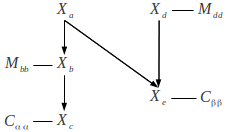
\includegraphics[width=0.49\linewidth]{system-graph.png}
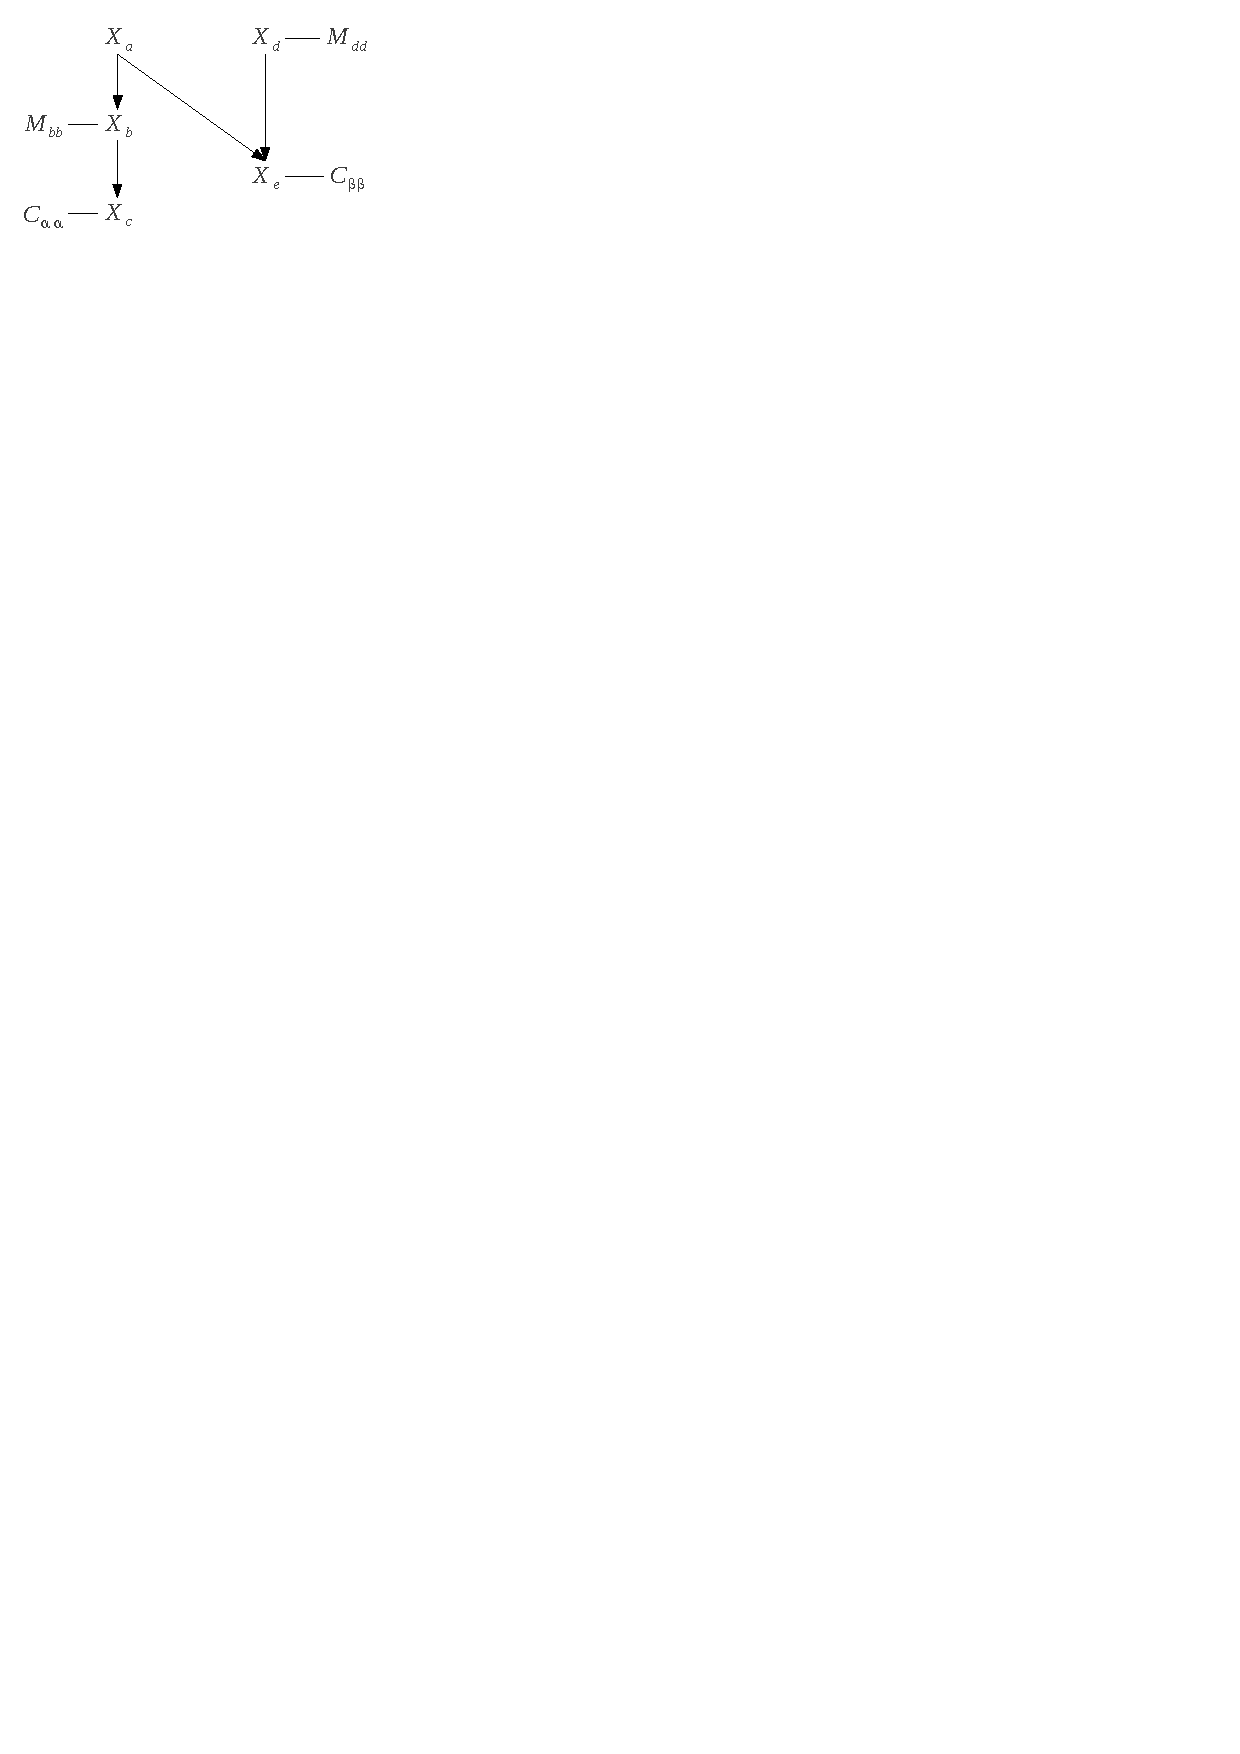
\includegraphics[clip,trim= 0mm 255mm 145mm 0mm,width=0.49\linewidth]{system-graph.pdf}
\caption{Example of mechanical system structure. The $X$ represent mechanical states, while the arrows represent the kinematic hierarchy, and the plain lines represent components acting on the states.}
\label{fig system graph}
\end{figure}


The corresponding equation system has the block structure shown in the right of Figure~\ref{fig system matrix}.
The main blocks of the equation system are highlighted in grey rectangles. The $J$ matrices are the mapping matrices. The bottom row has two mappings, since the state $X_e$ impacted by compliance $\beta$ depends on two parent states.
\begin{figure}
\centering
 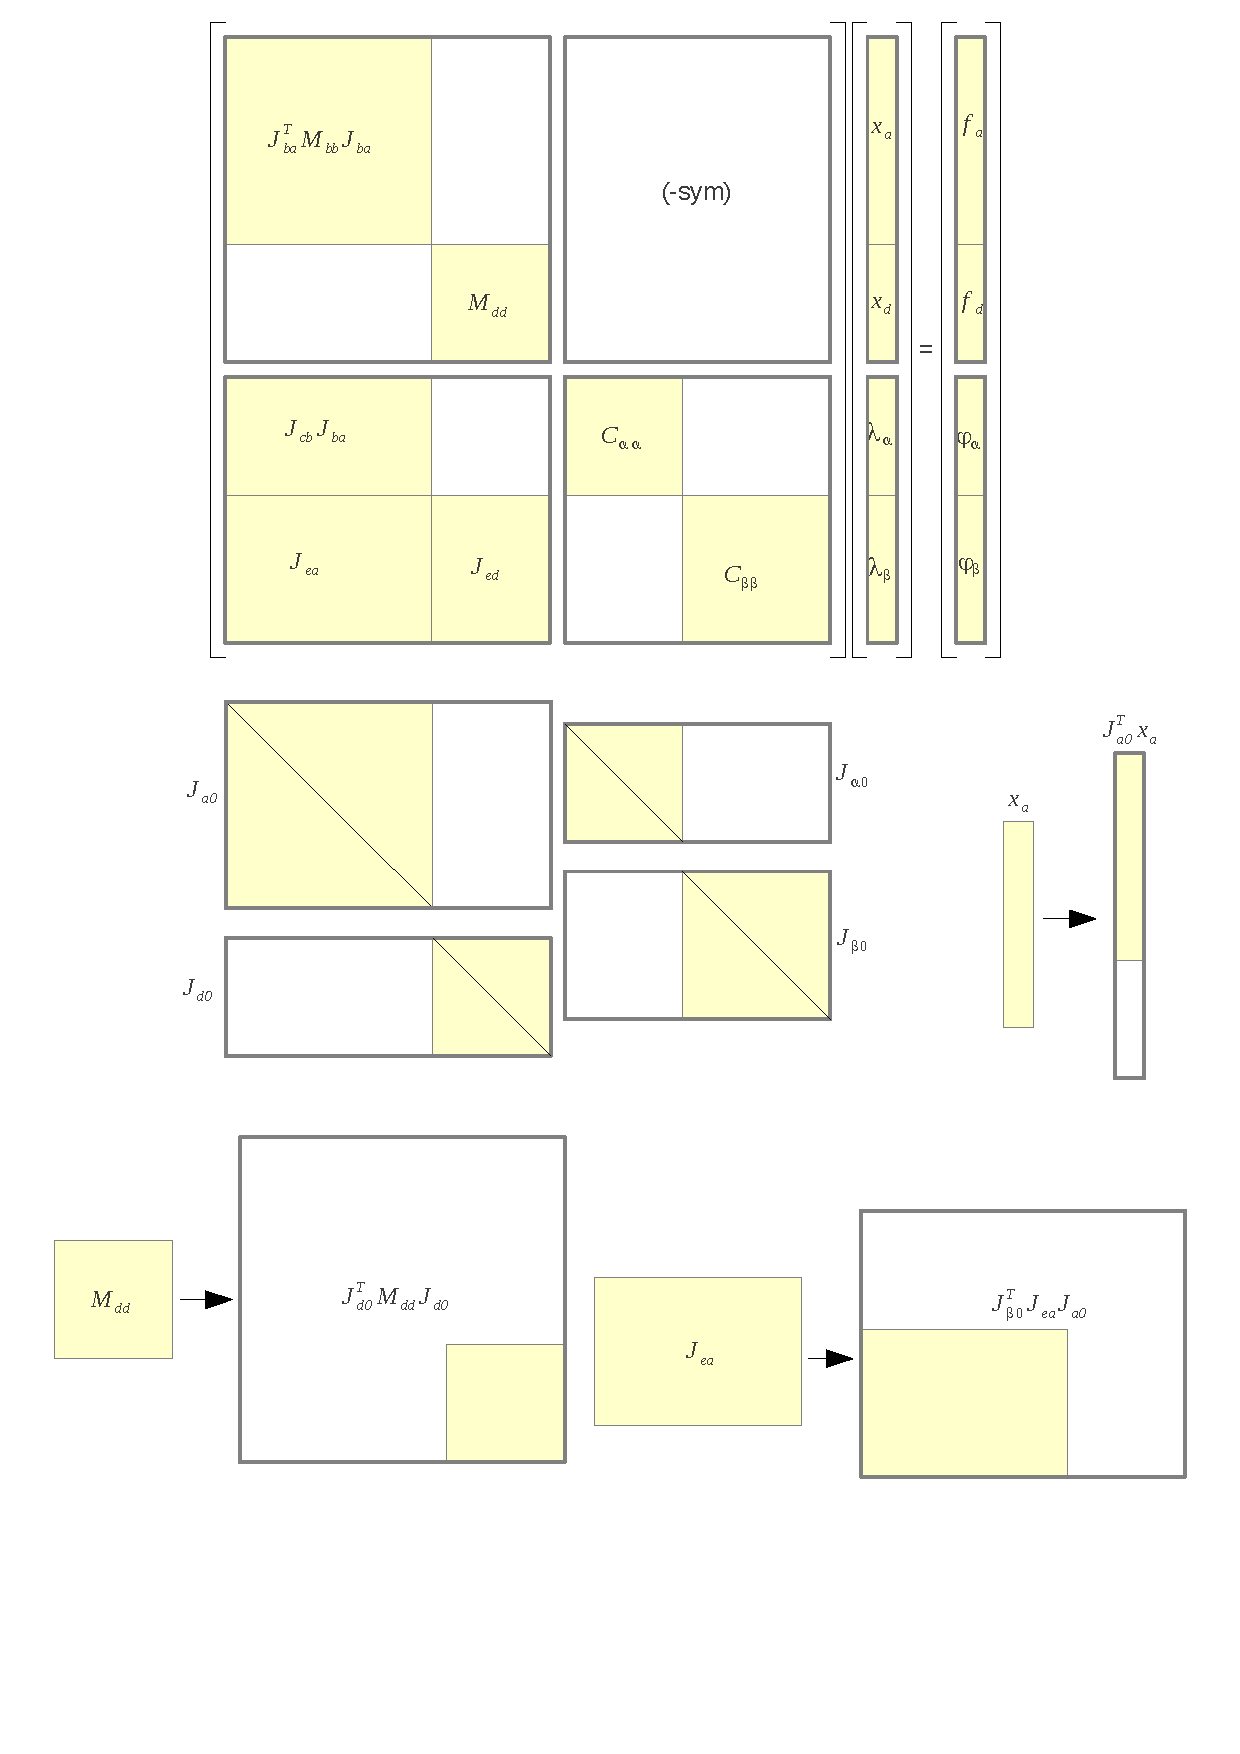
\includegraphics[clip,trim=5mm 185mm 40mm 0mm,width=0.7\linewidth]{system-bigmatrix.pdf}
\caption{Block view of the equation~\ref{eq abstract system} applied to the system of Figure~\ref{fig system graph}, with non-null blocks highlighted in yellow.}
\label{fig system matrix}
\end{figure}


The assembly of local matrices and vectors to the global matrices and vectors which compose the system is performed using shift matrices, as illustrated in Figure~\ref{fig shifting}.
Shift matrices $J_{*0}$, shown in the top of the figure, are composed of identity matrices (represented with a diagonal in a block) and null blocks. They can be used to implement the shifting of vector entry indices from local to global. 
\begin{figure}
\centering
%  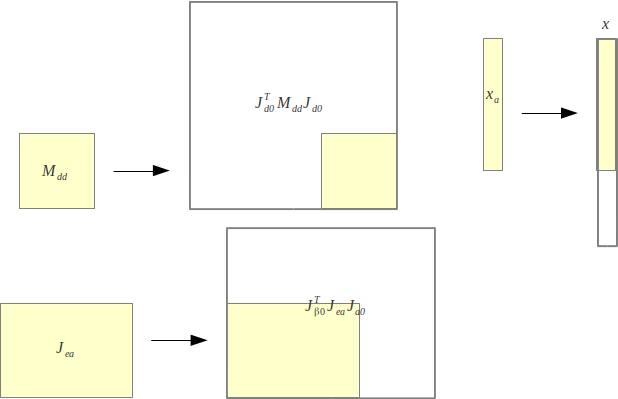
\includegraphics[width=0.69\linewidth]{system-shift.png}
 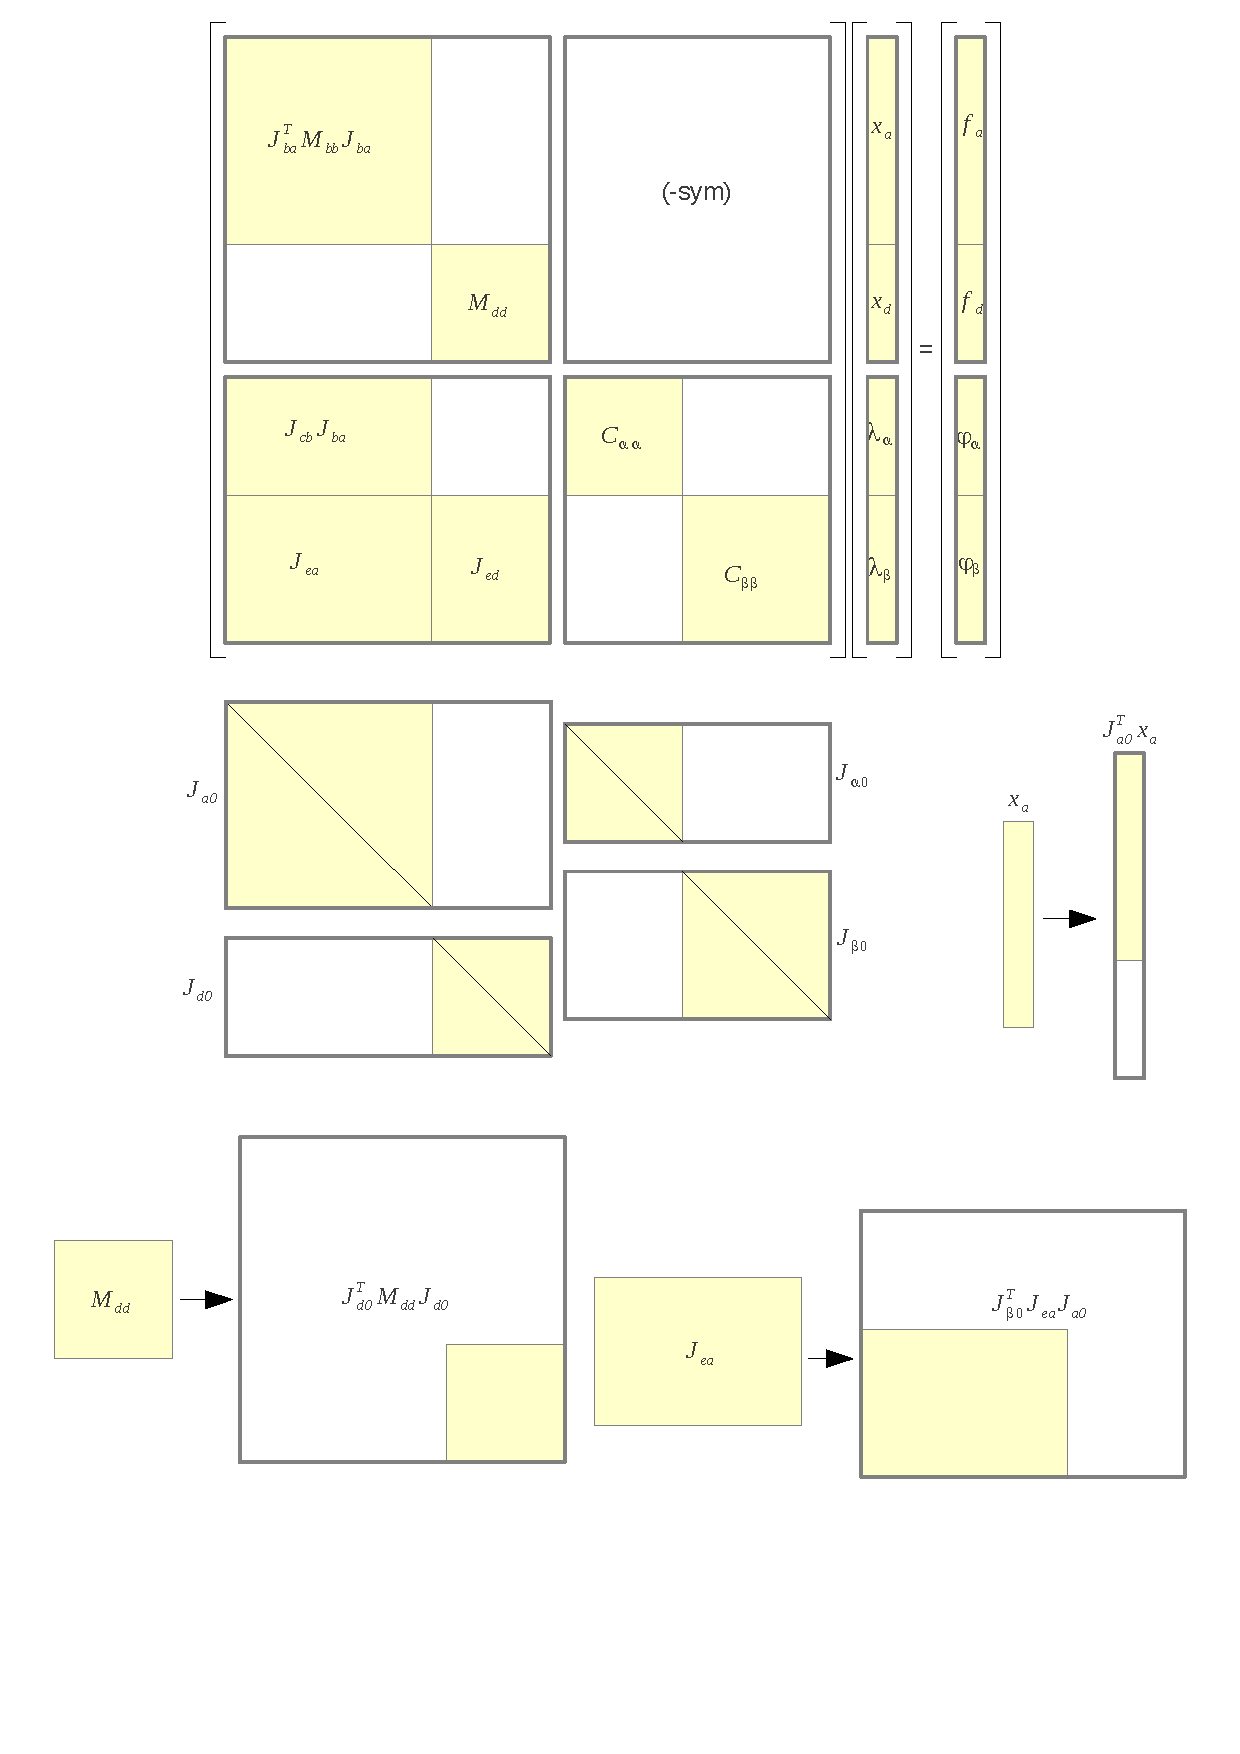
\includegraphics[clip,trim=0mm 40mm 0mm 115mm,width=0.89\linewidth]{system-bigmatrix.pdf}
\label{fig shifting}
\caption{Shift matrices $J_{*0}$ are used to place blocks within global vectors and matrices. }
\end{figure}
The assembly is thus easily expressed as a sum of product of matrices, as illustrated in Figure~\ref{fig assembly}. 
While shifting values in dense arrays using matrix products is not efficient (vector assembly is actually implemented using shifted copies), the sum of matrix products is a reasonable implementation of sparse matrix assembly.
\begin{figure}
\centering
%  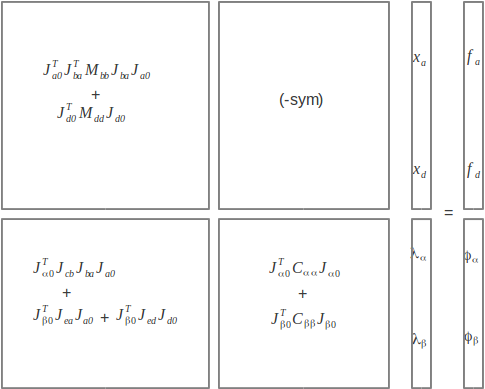
\includegraphics[width=0.6\linewidth]{system-assembly.png}
 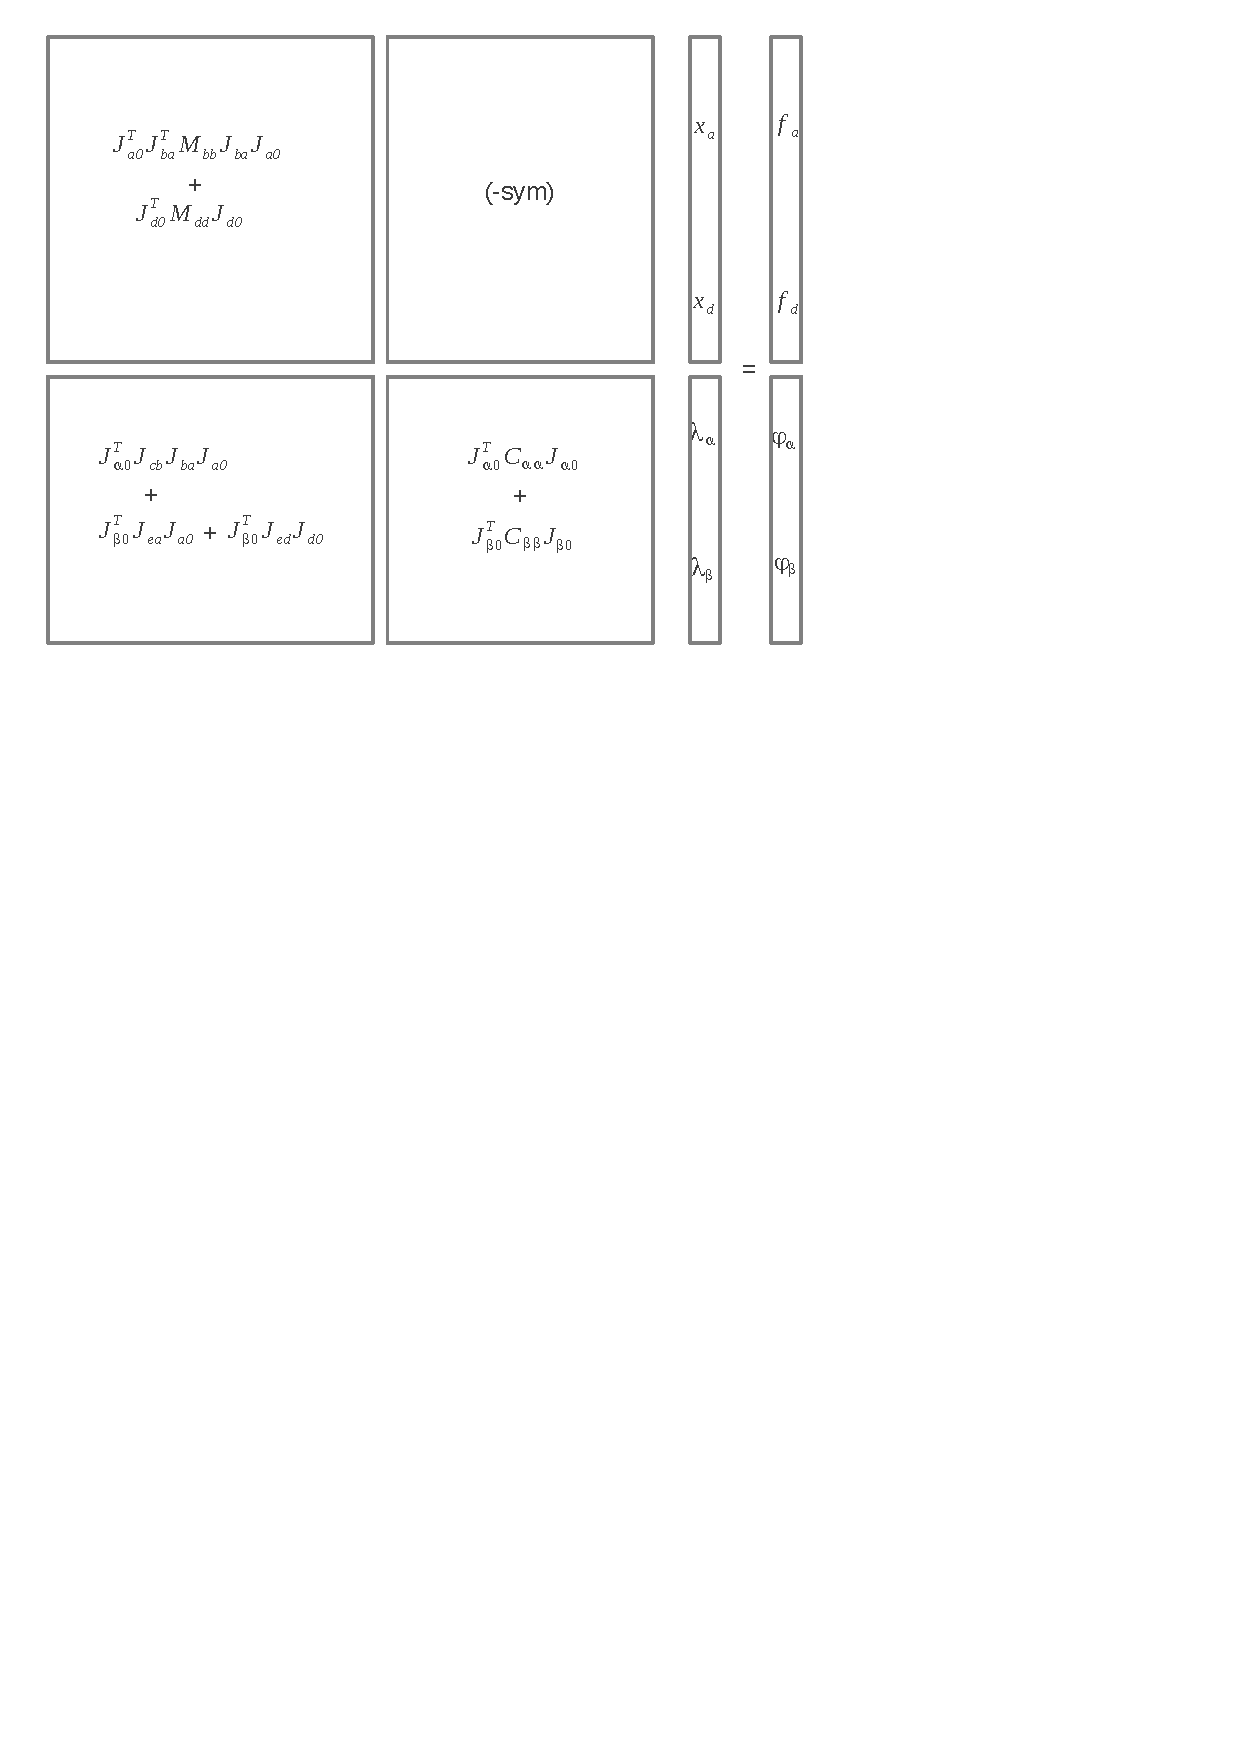
\includegraphics[clip,trim=5mm 185mm 70mm 5mm,width=0.6\linewidth]{system-assembly.pdf}
\caption{The assembly is performed by summing the global vectors and matrices obtained by shifting local vectors and matrices.}
\label{fig assembly}
\end{figure}


\section{Implementation} \label{sec implementation}

\subsection{Dependencies}
This plugin uses \texttt{Eigen} and \texttt{suitesparse}. Moreover, the test suite requires the \texttt{boost unit test framework}, see https://wiki.sofa-framework.org/wiki/UnitTesting  .

\subsection{Functions}

The virtual functions used for setting up the equation system are declared in BaseForceField.h, BaseMapping.h, BaseMass.h, BaseProjectiveConstraint.h, MechanicalParams.h.
They and documented in ``Experimental Compliance API'' documentation blocks of these files.


\subsection{BaseForceField functions}
ForceFields may be handled as forces or as soft constraints, as explained in Section~\ref{sec force or constraint}. 
The default behavior is to handle them as forces, and in this case their force is accumulated using a classical \texttt{MechanicalOperations::computeForce} operation, while their stiffness matrix is accumulated using the \texttt{getStiffnessMatrix} briefly described below.
\begin{itemize}
 \item \texttt{getComplianceMatrix} returns NULL if the ForceField is to be handled as a traditional force function, while it returns a pointer to a compliance matrix if it is to be handled as a constraint.
 \item \texttt{addForc}e is used to accumulate the force in the right-hand term. This function is not specific to the \textit{Compliant} plugin. This should do nothing when the force must be handled as a constraint.
 \item \texttt{getStiffnessMatrix} is the complement of \texttt{getCompliantMatrix}. If one retuns NULL, then the other must return a pointer to a matrix.
 \item \texttt{writeConstraintValue} is used to write the constraint violation $\violation$ in Eq.\ref{eq generalized constraint} when the ForceField is handled as a constraint.
 \item \texttt{getDampingRatio} is used in the constraint case, and corresponds to parameter $ \dampingratio$ in Eq.\ref{eq generalized constraint}
\end{itemize}

\subsubsection{BaseMapping functions}
\begin{itemize}
 \item \texttt{getJs} returns a list of Jacobian matrices, one for each parent of the mapping. Typical mappings have only one parent, but MultiMappings have several ones.
 \item \texttt{getKs} returns a list of stiffness matrices, one for each parent. These correspond to geometric stiffness, i.e. change of forces due to mapping nonlinearity, like \texttt{addDJT} in the traditional API. \textbf{\begin{large}TODO:                                                                                                                                                                                                                                       \end{large}} refine this, to also return off-diagonal terms in MultiMappings. 
\end{itemize}

\subsubsection{BaseMass functions}
\begin{itemize}
 \item \texttt{addMToMatrix} to create the mass matrix. This function is not specific to the \textit{Compliant} plugin.
\end{itemize}

\subsection{BaseProjectiveConstraint functions}
\begin{itemize}
 \item \texttt{projectMatrix} replaces a matrix with one corresponding to the same linear operator, projected to cancel, out the forbidden directions. 
\end{itemize}

\subsection{MechanicalParams functions}
\begin{itemize}
 \item \texttt{implicitVelocity} is the $\alpha$ parameter in the implicit velocity integration of Eq.\ref{eq ode velocity}.
 \item \texttt{implicitPosition} is the $\beta$ parameter in the implicit position integration of Eq.\ref{eq ode position}.
\end{itemize}


\section{Alternative model} \label{sec alternative model}
To allow more flexibility in the definition of damping in the compliance approach, the following variant is possible.
We replace eq.~\ref{eq generalized constraint} with the following.
\begin{equation}\label{eq generalized damped constraint}
\lam = - \C^{-1} \violation - \D \dviolation
\end{equation}
where $\violation$ and $\dviolation$ are vectors, and $\C$ and $\D$ symmetric matrices.
This allows us to define non-uniform damping coefficients.
We rewrite eq.~\ref{eq bottom} as:
\begin{equation}
 \label{eq bottom alt}
 \alpha( h \beta \I + \C \D) \J \dv + \C \avlam = -\violation - \alpha(h\I + \C\D )\dviolation
\end{equation}
where $\I$ is the identity matrix of the appropriate size.
Unfortunately, the diagonal matrix in the left of $\J$ in the term on $\dv$ now makes the Schur complement unsymmetric. Therefore, we have not implemented this approach.



\section{Additional Notes}
\label{sec:additional notes}

\newcommand{\component}[1]{\texttt{#1}}
\newcommand{\compopt}[2]{\texttt{#1}=''#2''\\}

The initial implementation of the compliance framework is provided by
\component{ComplianceSolver}, which performs system assembly, system
solves and time-stepping. It uses a sparse Cholesky solver and is able
to handle bilateral constraints only.

With time, this component has been broken down to the following
components:

\begin{itemize}
\item \component{AssembledSolver}, which performs system assembly
  (through an internal \component{AssemblyVisitor}) and
  time-stepping.
\item \component{KKTSolver}, which performs the KKT solve associated
  with an \component{AssembledSystem}, itself provided by the
  \component{AssembledSolver} though its internal
  \component{AssemblyVisitor}. 
\end{itemize}

\component{KKTSolver} is a virtual base class implemented in
\component{MinresSolver} and \component{LDLTSolver} for bilateral
constraints. The CompliantDev plugin contains additional KKT solvers
for unilateral and frictional constraints.

We now give a quick user documentation for the above components.

\subsection{AssembledSolver}

This component implements a linearized implicit Euler solver. The KKT
system is first assembled by an \component{AssemblyVisitor}, and
factorized by the \component{KKTSolver}.

The right-hand-side is then computed depending on constraint
stabilization and order of resolution, and the \component{KKTSolver}
provides system solves.

At the end of the time-step, velocities are updated and the system is
stepped forward. Optionally, one can propagate the computed Lagrange
multipliers upwards in the scene graph at the end of the time step in
the \emph{force} state vector for easy access.

\subsubsection{Order of Resolution}

\compopt{use\_velocity}{\textbf{true}, false}

Formulates the system at the velocity level. Acceleration is used
otherwise. This is mostly for debugging purpose, unless warm-starts
are disabled (see below).

\subsubsection{Warm Starts}

\compopt{warm\_start}{\textbf{true}, false}

Warm starts iterative solvers with previous velocity/lambda (velocity-level). At the
acceleration level, only the lambda are used.

When disabled and used with iterative solvers and premature exit, this
biases the solution towards zero, thus this results in numerical
damping with velocity-level.

This is mostly for debugging purpose.

\subsubsection{Constraint Stabilization}

\compopt{stablization}{\textbf{false}, true}

Performs simple constraint stabilization. This causes an additional
KKT solve during the time step.

You need to add a \component{Stabilization} component next to any
compliance you wish to stabilize. Only use with zero-compliance
(holonomic constraints).

TODO more, example

\subsection{Lagrange Multiplier Propagation}

\compopt{propagate\_lambdas}{\textbf{false}, true}

Optionally propagate/aggregate Lagrange multipliers from compliant
DOFs to independent DOFs at the end of the time step. This erases the
\emph{force} state vector.

TODO example

\subsection{LDLTSolver}

no options 

TODO more

\subsection{MinresSolver}

\compopt{iterations}{\textbf{false}, true}

iteration count

\compopt{precision}{\textbf{1e-8}}

residual norm threshold

\compopt{relative}{\textbf{true}, false}

use relative precision, otherwise absolute


TODO parallel ?
TODO schur complement ?

TODO better description

